% Snowflake Data Engineering — Chapter 10 | original manuscript draft
% Author: Arman Golbidi | Editorial snapshot: 22 October 2026
% Compile: xelatex -interaction=nonstopmode -halt-on-error Snowflake_Data_Engineering_Chapter_08.tex
% Trim: 178 x 254 mm; margins inside 23 mm / outside 17 mm / top-bottom 19 mm.
% Body: 10.75 pt / 13.65 pt leading = 1.27 line-height ratio; code: 8.75 pt.
\documentclass[11pt,twoside]{article}
\usepackage[paperwidth=178mm,paperheight=254mm,inner=23mm,outer=17mm,top=19mm,bottom=19mm,headheight=5mm,headsep=4mm,footskip=9mm]{geometry}
\usepackage{fontspec}
\setmainfont{LibertinusSerif-Regular.otf}[BoldFont=LibertinusSerif-Bold.otf,ItalicFont=LibertinusSerif-Italic.otf,BoldItalicFont=LibertinusSerif-BoldItalic.otf]
\setsansfont{LibertinusSans-Regular.otf}[BoldFont=LibertinusSans-Bold.otf,ItalicFont=LibertinusSans-Italic.otf]
\setmonofont{LibertinusMono-Regular.otf}[Scale=0.91]
\usepackage[english]{babel}
\usepackage{microtype}
\usepackage{setspace}
\setstretch{1.0}
\usepackage{titlesec,enumitem,tabularx,array,booktabs,needspace,fancyhdr,lastpage}
\usepackage[most]{tcolorbox}
\usepackage{tikz}
\usetikzlibrary{arrows.meta,positioning,fit,shapes.misc,calc}
\usepackage{listings}
\usepackage{xcolor}
\usepackage{hyperref}
\usepackage{amsmath}
\hypersetup{colorlinks=true,urlcolor=steelblue,linkcolor=steelblue,pdfauthor={Arman Golbidi},pdftitle={Snowflake Data Engineering - Chapter 10: ETL/ELT Pipelines, dbt, and Delivery Workflows},pdfsubject={English technical book manuscript, tenth chapter, 178 x 254 mm}}
\definecolor{navy}{HTML}{15334A}
\definecolor{steelblue}{HTML}{17779B}
\definecolor{teal}{HTML}{12888A}
\definecolor{lightblue}{HTML}{ECF5F7}
\definecolor{papergray}{HTML}{F2F5F6}
\definecolor{inkgray}{HTML}{4A5862}
\definecolor{thinrule}{HTML}{CBD7DB}
\AtBeginDocument{\color{navy}\fontsize{10.75}{13.65}\selectfont}
\setlength{\parindent}{0pt}
\emergencystretch=2.5em
\setlength{\parskip}{3.3pt plus 0.7pt minus 0.6pt}
\setlist[itemize]{leftmargin=4mm,itemsep=1pt,topsep=2pt,parsep=0pt}
\setlist[enumerate]{leftmargin=5mm,itemsep=1pt,topsep=2pt}
\titleformat{\section}{\sffamily\bfseries\color{navy}\fontsize{14}{17}\selectfont}{}{0pt}{}
\titlespacing*{\section}{0pt}{8pt}{4pt}
\titleformat{\subsection}{\sffamily\bfseries\color{steelblue}\fontsize{10.8}{13}\selectfont}{}{0pt}{}
\titlespacing*{\subsection}{0pt}{5pt}{1pt}
\newcommand{\topic}[2]{\subsection*{#1\quad #2}}
\newcommand{\repo}[2]{\par\begingroup\fontsize{8.0}{9.6}\selectfont\sffamily\color{inkgray}\textbf{Project reference:} \href{#2}{#1}. \textit{Not independently executed; rights review pending.}\par\endgroup}
\newtcolorbox{insight}[1][]{enhanced,breakable,colback=lightblue,colframe=thinrule,boxrule=.45pt,arc=1.3mm,left=2.8mm,right=2.8mm,top=1.8mm,bottom=1.8mm,before skip=5pt,after skip=5pt,#1}
\newtcolorbox{whitebox}[1][]{enhanced,breakable,colback=papergray,colframe=thinrule,boxrule=.35pt,arc=1mm,left=2.6mm,right=2.6mm,top=1.5mm,bottom=1.5mm,before skip=4pt,after skip=5pt,#1}
\lstdefinestyle{chaptercode}{basicstyle=\ttfamily\fontsize{8.75}{10.7}\selectfont,backgroundcolor=\color{papergray},frame=single,framerule=.35pt,rulecolor=\color{thinrule},breaklines=true,columns=fullflexible,keepspaces=true,showstringspaces=false,aboveskip=5pt,belowskip=5pt,xleftmargin=2mm,xrightmargin=1mm,framexleftmargin=2mm,framexrightmargin=1mm}
\lstset{style=chaptercode}
\pagestyle{fancy}
\fancyhf{}
\fancyhead[LE]{\sffamily\fontsize{7.6}{9}\selectfont\color{inkgray}\textsc{Snowflake Data Engineering}}
\fancyhead[RO]{\sffamily\fontsize{7.6}{9}\selectfont\color{inkgray}\textsc{10 / dbt \& Delivery}}
\fancyfoot[LE,RO]{\sffamily\bfseries\fontsize{8.2}{9}\selectfont\color{steelblue}\thepage}
\fancyfoot[LO,RE]{\sffamily\fontsize{7.6}{9}\selectfont\color{inkgray}Arman Golbidi \quad | \quad Chapter 10}
\renewcommand{\headrulewidth}{0.35pt}
\renewcommand{\footrulewidth}{0pt}
\setcounter{page}{171}
\raggedbottom

\begin{document}
% PAGE 171
{\sffamily\bfseries\fontsize{9}{11}\selectfont\color{steelblue} CHAPTER 10 \hfill ENGINEERING / TRANSFORMATION DELIVERY}\par\vspace{3mm}
{\sffamily\bfseries\fontsize{21.2}{24.5}\selectfont\color{navy} ETL/ELT Pipelines, dbt,\\and Delivery Workflows}\par\vspace{2mm}
{\sffamily\fontsize{11.1}{14}\selectfont\color{steelblue} A passing transformation is not yet a deployable data product}\par\vspace{3mm}
\begin{insight}\textbf{An accurate dashboard can be one deployment away from a silent failure.}\par
At 08:15, Finland Energy Analytics reports 66.000~MWh from six accepted technology readings. At 08:20, a developer adjusts an incremental filter. The next deployment succeeds, but a late correction is ignored; the dashboard becomes stale while every task remains green. The team has a SQL query, but not yet a trustworthy delivery workflow. Who owns the source contract? Which test would have failed? Can an operator restore the last accepted result without erasing the corrected records?
\end{insight}
The previous chapters built ingestion, revision handling, incremental state and Python transformations. This chapter adds an engineering discipline around them: \emph{declarative transformation models, source contracts, documented lineage, controlled execution and safe release}. We use dbt to make these concerns inspectable. Neither dbt nor an orchestration service automatically guarantees correctness; the guarantees come from explicit tests, sound keys, reliable source semantics and operational procedures.
\begin{whitebox}\textbf{Learning outcomes}\par
After this chapter you can: contrast ETL and ELT; organise bronze, silver and gold models; configure a minimal Snowflake dbt project; implement source/model tests; distinguish incremental state from history; evaluate Snowflake Tasks and external orchestrators; configure a conservative CI pipeline; apply freshness and quality gates; and document a reversible release.\end{whitebox}
\textbf{Prerequisites.} Chapters~4, 8 and 9, Git, SQL and basic Python. Cloud exercises need a restricted Snowflake role, approved warehouse, and dbt adapter. The companion includes a \textbf{zero-cloud Python oracle}; the dbt project is prepared for a separately approved integration test, not claimed executed here.
\begin{center}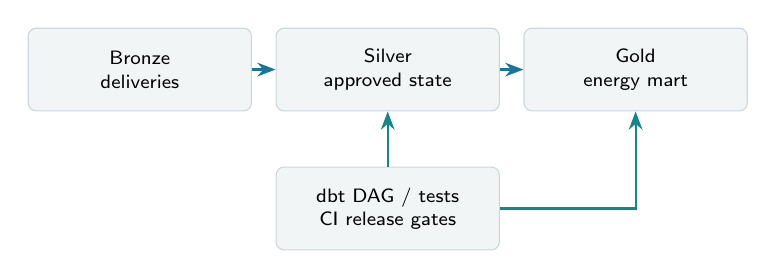
\begin{tikzpicture}[>=Stealth,every node/.style={font=\sffamily\fontsize{7.5}{8.5}\selectfont},n/.style={draw=thinrule,rounded corners=1mm,fill=papergray,align=center,text width=26mm,minimum height=10.5mm}]
\node[n](a){Bronze\\deliveries}; \node[n,right=3mm of a](b){Silver\\approved state};\node[n,right=3mm of b](c){Gold\\energy mart};
\node[n,below=7mm of b](d){dbt DAG / tests\\CI release gates};
\draw[->,thick,steelblue](a)--(b);\draw[->,thick,steelblue](b)--(c);\draw[->,thick,teal](d)--(b);\draw[->,thick,teal](d)-|(c);
\end{tikzpicture}\\{\fontsize{8}{9}\selectfont\color{inkgray}Figure 10.1. Correctness evidence and change controls surround the transformation path.}\end{center}
\newpage
% PAGE 172
\section*{10.1\quad ETL versus ELT: architecture and trade-offs}
\topic{10.1.1}{ETL versus ELT execution paths}
\textbf{Extract--transform--load (ETL)} transforms data before it enters the analytical destination; \textbf{extract--load--transform (ELT)} lands permitted source data and performs subsequent transformations within or adjacent to the destination. These acronyms describe \emph{execution order}, not the quality of the pipeline. Both can validate, protect privacy and maintain lineage; both can also do those things poorly.

Take twelve synthetic revision events from Chapter~9. An ETL service could parse the CSV, reject invalid measurements, apply winning revisions, and then load six approved energy facts. Under ELT, the same event deliveries are first written into a bronze relation, while Snowflake SQL models perform checks, deduplication and curation. The business outcome must be compared at a specified grain, not inferred from architecture labels.
\begin{center}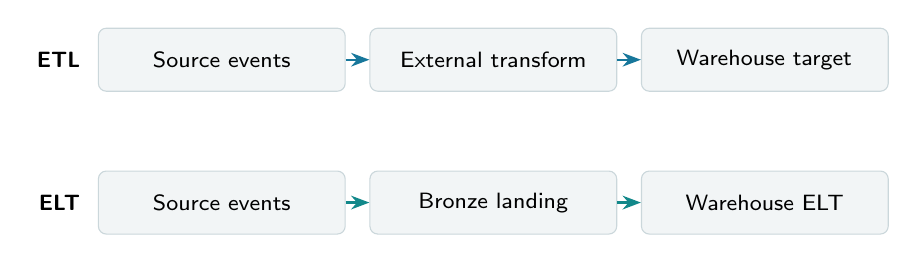
\begin{tikzpicture}[>=Stealth,every node/.style={font=\sffamily\fontsize{7.8}{9}\selectfont},n/.style={draw=thinrule,rounded corners=1mm,fill=papergray,align=center,minimum height=8mm,text width=29mm}]
\node[n](a){Source events};\node[n,right=3mm of a](b){External transform};\node[n,right=3mm of b](c){Warehouse target};
\draw[->,steelblue,thick](a)--(b);\draw[->,steelblue,thick](b)--(c);
\node[n,below=10mm of a](d){Source events};\node[n,right=3mm of d](e){Bronze landing};\node[n,right=3mm of e](f){Warehouse ELT};
\draw[->,teal,thick](d)--(e);\draw[->,teal,thick](e)--(f);
\node[left=1mm of a,font=\sffamily\bfseries\fontsize{8}{9}\selectfont]{ETL};\node[left=1mm of d,font=\sffamily\bfseries\fontsize{8}{9}\selectfont]{ELT};
\end{tikzpicture}\\{\fontsize{8}{9}\selectfont\color{inkgray}Figure 10.2. The key distinction is where the transformation boundary falls.}\end{center}
\textbf{Preserve an audit trail.} Loading a raw event does not mean every field should be retained indefinitely. A bronze zone should enforce approved retention, access and masking requirements. Where the incoming payload contains sensitive information, extract-and-redact before persistence may be a better architecture. An analytical platform is not a justification for unrestricted raw-data accumulation.
\begin{whitebox}\textbf{Decision rule}\par
If a source must be cleansed or de-identified before crossing a legal or contractual boundary, ETL or a privacy-preserving hybrid may be mandatory. If data can be landed safely and the main transformations are relational, ELT often simplifies lineage and makes compute elastic. Decide from constraints; do not select an acronym first.\end{whitebox}
\textbf{Check.} Which stage holds the first durable copy of a source record in each design? Where would you quarantine an invalid negative MWh value?
\newpage
% PAGE 173
\topic{10.1.2}{Pushdown and platform trade-offs}
\emph{Pushdown} means delegating operations to a compute engine near the relevant data rather than exporting intermediate rows to a separate process. A dbt SQL model normally executes through the destination adapter; Snowflake evaluates the SQL on its compute. This avoids unnecessary client materialisation for ordinary joins and aggregates. It does \emph{not} mean external engines are obsolete: specialised libraries, contractual boundaries, or source-side API restrictions may require upstream processing.

For the energy example, aggregating \texttt{SUM(ENERGY\_MWH)} by \texttt{INTERVAL\_UTC} is naturally pushed into a Snowflake SQL model. Parsing a proprietary binary instrument message, by contrast, may warrant a narrowly scoped extraction service. An engineer should record the trust boundary and data movement in either design.
\begin{lstlisting}[language=SQL,caption={Warehouse-side gold calculation; assumes accepted silver rows.}]
SELECT interval_utc, SUM(energy_mwh) AS total_mwh
FROM analytics.silver_energy
GROUP BY interval_utc;
\end{lstlisting}
The main trade-offs are \textbf{transfer cost}, \textbf{replay capability}, \textbf{compute isolation}, \textbf{governance}, and \textbf{operational complexity}. A cloud warehouse can scale compute separately from storage, yet badly selected warehouse sizes and repeated full scans can still be expensive. An external compute engine may be cheaper for a particular transformation but create operational expense in scheduling, credentials, logs and recovery.
\begin{center}\renewcommand{\arraystretch}{1.12}\begin{tabularx}{\linewidth}{@{}p{31mm}XX@{}}\toprule
\textbf{Dimension}&\textbf{ETL before loading}&\textbf{ELT within Snowflake}\\\midrule
Data movement&Potential pre-load processing and copies&Raw landing, then in-platform queries\\
Lineage&Must connect two execution systems&dbt graph plus source/load evidence\\
Failure recovery&Replay external transform and upload&Rebuild downstream objects from retained bronze\\
Compliance&Can redact before destination&Needs landing permissions and retention policy\\
Economics&External runtime and transport charges&Warehouse and storage charges\\\bottomrule\end{tabularx}\end{center}
\begin{insight}\textbf{Failure case: the appealing six-row benchmark}\par
Do not compare a local process that reads six rows with a warehouse pipeline that checks and processes a million. Benchmark the same input, identical business semantics, matching output, relevant data-transfer boundaries and fully itemised cost.\end{insight}
\textbf{Check.} When would replacing an ELT SQL aggregate with a pandas download worsen observability even if elapsed time falls in a tiny demo?
\newpage
% PAGE 174
\topic{10.1.3}{Selecting a design for maintainability}
A maintainable design places each rule where its meaning is obvious and its behaviour is independently testable. For our energy project, separate \emph{delivery validation} (may this event be accepted?), \emph{state resolution} (which revision wins?) and \emph{analytical representation} (which measure and grain do consumers see?). Mixing all three inside a long SQL statement may deliver the expected number but makes drift, deletions and late corrections difficult to investigate.

Write a short architecture decision record (ADR). State the requirements, alternatives, reasons, constraints and a trigger to revisit the decision. Do not claim that ELT always reduces complexity: dbt can create its own configuration, dependency, deployment and observability work. The objective is an explainable path to a stable output.
\begin{whitebox}\textbf{ADR-010: illustrative decision}\par
\textbf{Context:} permitted synthetic events arrive in small batches; engineers own Snowflake SQL and Git. \textbf{Decision:} retain an audited bronze history, transform approved revisions with dbt, publish a gold mart; use a local Python oracle in CI. \textbf{Rejected default:} exporting all bronze rows to a local Python job. \textbf{Revisit when:} required latency, data volume or regulatory obligations change materially. \textbf{Risk:} source freshness and Snowflake SQL validation must be checked independently.\end{whitebox}
\begin{lstlisting}[caption={A concise acceptance contract for the running example.}]
Grain:     provider + technology + interval_utc
Revision:  highest valid positive revision wins
Delete:    latest DELETE makes its key invisible
Value:     finite and >= 0 MWh for UPSERT
Oracle:    6 rows; SUM(energy_mwh) = 66.000
Proof:     source tests + model tests + offline oracle
\end{lstlisting}
An acceptance contract is also a \emph{boundary for change}. If the business later wants both corrected and original measurements displayed, that is a new semantic requirement, not a one-line enhancement. Its consequences may include an event-history table, revised gold grain and new tests.
\repo{P108: Astronomer ETL/ELT with Airflow and Snowflake}{https://github.com/astronomer/etl-elt-airflow-snowflake}
\textbf{Check.} What would make an ELT-first design inappropriate even if the Snowflake code is technically correct?
\newpage
% PAGE 175
\section*{10.2\quad Bronze, silver, and gold transformation layers}
\topic{10.2.1}{Raw bronze ingestion}
A \emph{bronze layer} preserves approved source deliveries, their provenance and enough detail to explain what happened. In this book the small input is a revisioned energy-event CSV. It deliberately includes a repeated event ID, an older hydro reading, a logical deletion, a negative quantity and a zero revision. A source delivery is not automatically a business fact: bronze records may be incomplete, invalid or superseded.

A useful bronze contract records the source identifier, delivery timestamp, file or batch reference, schema version, ingestion outcome and retention rules. Snowflake file metadata can help trace staged loads; application records should not pretend every connector exposes exactly the same fields. Stable event IDs and batch lineage are especially helpful during replay.
\begin{lstlisting}[language=SQL,caption={Illustrative bronze landing structure.}]
CREATE TABLE IF NOT EXISTS RAW_ENERGY_EVENTS (
  event_id VARCHAR, provider VARCHAR,
  technology VARCHAR, interval_utc VARCHAR,
  revision VARCHAR, energy_mwh VARCHAR,
  operation VARCHAR, source_batch VARCHAR,
  ingested_at TIMESTAMP_LTZ DEFAULT CURRENT_TIMESTAMP()
);
\end{lstlisting}
\textbf{Why text in bronze?} Retaining malformed numeric strings can be useful for diagnosis. At silver, a failed cast is a quality event; at bronze, the original payload is evidence. If compliance rules disallow persisting a field, exclude or mask it before this point.

\begin{insight}\textbf{Common error: treating ingestion success as analytical validity}\par
A batch can load completely while containing a negative MWh value. Loading, parsing, validation, correction handling and publication are separate states. A dashboard must never infer quality solely from the absence of a COPY error.\end{insight}
\textbf{Practical task.} Identify the three fields you would require for answering ``which file supplied this incorrect nuclear measurement?'' How would you prevent repeated transfers from doubling a reported total?
\newpage
% PAGE 176
\topic{10.2.2}{Validated silver transformation}
Silver provides a stable, explicitly defined analytical contract. For our energy stream, the rules are: reject negative quantities and invalid revisions, collapse exact replay events, identify the highest accepted revision for each provider--technology--UTC interval, and exclude a key whose winning event is a DELETE. These steps must be consistent with earlier chapters; this chapter does not quietly alter their meanings.
\begin{lstlisting}[language=SQL,caption={Core revision-resolution pattern; abbreviated for print.}]
WITH valid AS (
  SELECT * FROM raw_energy_events
  WHERE TRY_TO_NUMBER(revision) >= 1
    AND TRY_TO_DECIMAL(energy_mwh,18,3) >= 0
), latest AS (
  SELECT *, ROW_NUMBER() OVER (
    PARTITION BY provider, technology, interval_utc
    ORDER BY TRY_TO_NUMBER(revision) DESC, event_id DESC
  ) AS rn FROM valid
)
SELECT * FROM latest
WHERE rn = 1 AND UPPER(operation) = 'UPSERT';
\end{lstlisting}
This is an instructional fragment, not a full conflict policy. A real pipeline must also check identical event IDs, equal-revision disagreements, timestamp format, allowed operations and null keys. The companion project implements those checks around the printed SQL. If two distinct readings claim the same business key and revision, selecting an arbitrary winner risks silent corruption: quarantine the conflict and request source-owner resolution.
\topic{10.2.3}{Business-ready gold marts}
Gold models expose consumer-oriented measures and grain. Our \texttt{fct\_energy\_hourly} contains one row per UTC interval and technology, with a sum of accepted MWh. A separate daily roll-up should use a documented calendar convention; converting UTC to \texttt{Europe/Helsinki} may create 23- or 25-hour local days around daylight-saving changes. Never mix local date and UTC interval silently.
\begin{lstlisting}[language=SQL,caption={A gold measure with explicit grain.}]
SELECT interval_utc, technology,
       SUM(energy_mwh) AS energy_mwh
FROM silver_energy
GROUP BY interval_utc, technology;
\end{lstlisting}
\repo{P043: Snowflake retail analytics pipeline}{https://github.com/Snowflake-Labs/sfguide-building-retail-analytics-de-pipeline}
\textbf{Check.} Why should a downstream BI model query gold rather than recalculate the highest revision from arbitrary bronze deliveries?
\newpage
% PAGE 177
\section*{10.3\quad Structuring a dbt project for Snowflake}
\topic{10.3.1}{Core dbt project structure}
\emph{dbt} is a transformation framework in which SQL models, dependency declarations, tests, documentation and configuration form an auditable directed acyclic graph (DAG). The \texttt{ref()} function declares a dependency on another dbt model or seed; \texttt{source()} refers to a declared external relation. dbt compiles templated SQL, runs the relevant adapter queries and produces execution artifacts. It does not itself ingest files, create a complete incident response process or substitute for an external business contract.
\begin{lstlisting}[caption={Minimal repository tree in the companion archive.}]
dbt_project/
  dbt_project.yml
  profiles.example.yml
  seeds/energy_revisions.csv
  models/staging/stg_energy_events.sql
  models/intermediate/int_energy_current.sql
  models/marts/fct_energy_hourly.sql
  models/schema.yml
  tests/assert_fixture_total.sql
.github/workflows/offline-checks.yml
.github/workflows/manual-cloud-deploy.yml
\end{lstlisting}
The file \texttt{dbt\_project.yml} names the project, sets its profile and groups model defaults. A seed is a tiny CSV that dbt can load to a development database. It is convenient for a deterministic teaching fixture; it is not a recommended high-volume source-ingestion mechanism. Model names and directory structure should communicate responsibilities rather than mirror an organisation chart.
\begin{lstlisting}[caption={Simplified project configuration.}]
name: 'finland_energy_ch10'
version: '1.0.0'
config-version: 2
profile: 'finland_energy_ch10'
model-paths: ['models']
seed-paths: ['seeds']
test-paths: ['tests']
models:
  finland_energy_ch10:
    staging: {+materialized: view}
    intermediate: {+materialized: view}
    marts: {+materialized: table}
\end{lstlisting}
\textbf{Test what changes.} A source-file rename, a new macro or a model configuration update may change compiled SQL and dependency selection. Store source and configuration in Git, review both and capture artifacts for reproducibility. Avoid mixing credentials with model code.
\repo{P109: Getting started with dbt on Snowflake}{https://github.com/Snowflake-Labs/getting-started-with-dbt-on-snowflake}
\textbf{Check.} Why should a model reference \texttt{\{\{ ref('stg\_energy\_events') \}\}} rather than a hard-coded production schema?
\newpage
% PAGE 178
\topic{10.3.2}{Snowflake profiles and targets}
A dbt profile connects a selected target name to Snowflake account, database, schema, role and warehouse settings. Keep confidential values in a secret manager or environment variables; never commit tokens or passwords to a book repository. For a local dbt Core-style configuration, a credentials-free \texttt{profiles.example.yml} makes required names explicit while leaving values to the operator.
\begin{lstlisting}[caption={Environment-driven profile excerpt; no secrets provided.}]
finland_energy_ch10:
  target: dev
  outputs:
    dev:
      type: snowflake
      account: "{{ env_var('DBT_SNOWFLAKE_ACCOUNT') }}"
      user: "{{ env_var('DBT_SNOWFLAKE_USER') }}"
      authenticator: externalbrowser
      role: "{{ env_var('DBT_SNOWFLAKE_ROLE') }}"
      database: "{{ env_var('DBT_SNOWFLAKE_DATABASE') }}"
      warehouse: "{{ env_var('DBT_SNOWFLAKE_WH') }}"
      schema: CH10_DEV
      threads: 2
\end{lstlisting}
The choice of \texttt{externalbrowser} is illustrative for an interactive workstation, not a universal unattended CI authentication strategy. Service identities require approved noninteractive authentication and carefully scoped privileges. Test edition, account policies and adapter support before adopting any recipe from the internet.
\topic{10.3.3}{Separation of development and deployment}
A private development schema protects production objects from experiments. The production deployment identity should access only the schemas and compute needed for its tasks, not run as \texttt{ACCOUNTADMIN}. Define who can approve production changes, how expensive warehouse usage is limited and how a failed build prevents promotion. In a real installation, environment naming must also account for dbt's schema-generation behaviour: a custom schema name may be appended to the target schema rather than replace it, unless project macros change that convention.
\begin{whitebox}\textbf{Environment contract}\par
\textbf{Dev:} synthetic data, developer role, bounded credits, disposable schema. \textbf{CI:} isolated temporary namespace or approved selective-build strategy, no write permission to production tables. \textbf{Prod:} approved code, stable role, explicit build window, retained run artifacts and rollback owner.\end{whitebox}
\repo{P111: dbt and Snowflake hands-on lab}{https://github.com/dbt-labs/snowflake_sko_hol_2026}
\textbf{Check.} Which settings must differ between a developer's laptop and an unattended production job even if both compile identical SQL?
\newpage
% PAGE 179
\section*{10.4\quad Models, sources, tests, and documentation}
\topic{10.4.1}{Source declarations and models}
The semantic origin of a relation matters. In dbt, a source declaration makes the upstream object an explicit DAG node, while \texttt{ref()} gives downstream consumers a stable dependency on a managed model. Use a \emph{seed} only for this chapter's tiny synthetic fixture; a production pipeline would normally declare a landed bronze source whose freshness and ingestion owner are documented.
\begin{lstlisting}[caption={Selected YAML model properties; dbt Core-style syntax.}]
version: 2
models:
  - name: fct_energy_hourly
    description: "Accepted synthetic MWh by UTC hour and type"
    columns:
      - name: technology
        data_tests: [not_null]
      - name: energy_mwh
        data_tests: [not_null]
\end{lstlisting}
\topic{10.4.2}{Data tests and documented lineage}
A \emph{generic data test} checks a reusable condition: uniqueness, non-nullness, relationships or accepted values. A \emph{singular test} is an SQL query returning offending rows; an empty result normally means the test passed. Tests must match the model grain and domain. A total-mismatch test tied to an invented teaching fixture is appropriate in this chapter, but would be a harmful permanent rule for real Finnish energy statistics.
\begin{lstlisting}[language=SQL,caption={A fixture-only dbt singular test; zero rows means pass.}]
SELECT SUM(energy_mwh) AS observed_mwh
FROM {{ ref('fct_energy_hourly') }}
HAVING ABS(SUM(energy_mwh) - 66.000) > 0.0001;
\end{lstlisting}
Lineage is not simply a diagram. It should identify the business definitions used at each edge: event revision key, accepted values, UTC grain and publication contract. The DAG explains dependencies, while incident evidence identifies which source batch and model invocation produced a visible number.
\topic{10.4.3}{Build failures and acceptance criteria}
\texttt{dbt build} runs selected models and relevant tests, and failures must gate promotion rather than merely appear in logs. A SQL syntax error, a relationship-test failure and a missing upstream relation need distinct diagnostic procedures. \textbf{Source freshness is a separate operation}; do not claim a normal \texttt{dbt build} has necessarily checked it. The command names and supported properties should be verified against the pinned dbt Core/adapter versions used for release.
\repo{P112: dbt Core repository}{https://github.com/dbt-labs/dbt-core}
\textbf{Check.} Why does a passing \texttt{not\_null} test on \texttt{technology} not establish that exactly one current revision exists for each key?
\newpage
% PAGE 180
\section*{10.5\quad Incremental models and snapshot strategies}
\topic{10.5.1}{Incremental model configuration}
A dbt incremental model updates an existing destination rather than rebuilding it in full each time. The first run typically creates the table; subsequent runs apply a developer-defined source filter and adapter-specific incremental strategy. \texttt{unique\_key} is not a substitute for testing source uniqueness: duplicate rows in the update set can make a merge ambiguous, and repeated versions can silently corrupt current-state semantics.
\begin{lstlisting}[language=SQL,caption={Minimal incremental pattern; adapt to validated change-feed data.}]
{{ config(materialized='incremental',
          incremental_strategy='merge',
          unique_key='event_business_key') }}
SELECT * FROM {{ ref('stg_changes') }}
{% if is_incremental() %}
WHERE source_updated_at >= (
    SELECT DATEADD('hour',-2,MAX(source_updated_at))
    FROM {{ this }}
)
{% endif %}
\end{lstlisting}
The two-hour lookback is a \emph{design hypothesis}, not a general guarantee. Late corrections can arrive beyond it, and wall-clock update timestamps may not agree with source revision order. For critical energy data, retain a full history and document replay or rebuild conditions. Aggregate output must be recomputed for all affected keys, not merely append newly arrived increments.
\topic{10.5.2}{Snapshot and change-history techniques}
A snapshot records historical versions when a tracked relation changes. A snapshot is useful for mutable source rows that overwrite previous state and where point-in-time reconstruction matters. If an upstream event log already preserves every revision, a second snapshot may duplicate history and processing costs. The decision depends on audit requirements, source overwrite behaviour and the available change timestamp.
\topic{10.5.3}{Rebuild, reprocess, and schema drift}
\texttt{--full-refresh} is a powerful operational tool, not a harmless retry flag: rebuilding can consume substantial compute, alter object state and interact with consumers. A schema change should be evaluated against compatibility, dbt adapter behaviour and downstream contracts before activation. Always stage a full refresh and compare row counts, keys, totals, latency and access grants in an approved environment.
\begin{insight}\textbf{Failure mode: a late wind correction}\par
An incremental filter based only on maximum already-processed timestamp can drop a valid revision arriving today for last week's interval. Business time and ingestion time are separate coordinates. Carry a replay window or explicit affected-key strategy, and test it.\end{insight}
\repo{P113: incremental dbt reference}{https://github.com/arnoN7/dbt-incremental-stream}
\textbf{Check.} How would you approve a production full refresh?
\newpage
% PAGE 181
\section*{10.6\quad Native and external orchestration options}
\topic{10.6.1}{Native orchestration options}
Snowflake Tasks can schedule SQL actions and arrange task graphs inside the platform. They can also be triggered under supported conditions. Their strengths include a small operational footprint for platform-local work; their limitations depend on dependencies, retries, deployment workflow and the need to coordinate external systems. A Task does not replace dbt's model graph: one describes when work runs, while the other describes what transformations depend on what inputs.
\topic{10.6.2}{External schedulers and dependencies}
Airflow, Prefect and similar orchestration systems can coordinate downloads, validation, dbt commands, approvals and downstream notifications. They introduce an external state store, worker environment, permissions and another availability boundary. A pipeline that lands an API feed, validates raw contracts, runs dbt, checks freshness and publishes a BI artifact may benefit from such orchestration. A small warehouse-only transformation often does not need this additional platform.
\begin{center}\renewcommand{\arraystretch}{1.10}\begin{tabularx}{\linewidth}{@{}p{32mm}XX@{}}\toprule
\textbf{Dimension}&\textbf{Snowflake-native}&\textbf{External scheduler}\\\midrule
Primary domain&SQL / warehouse execution&Cross-system tasks and approvals\\
Dependency view&Task graph and history&Orchestrator DAG and run states\\
Credentials&Snowflake role boundaries&Secrets across several systems\\
Failure control&Task retry, history and alerts&Custom retry, backfill and alerts\\
Operations&Fewer moving parts for local tasks&Additional infrastructure lifecycle\\\bottomrule\end{tabularx}\end{center}
\topic{10.6.3}{Choosing based on reliability and operations}
List actual failure scenarios: network outage during input fetch, partial object deployment, a source schema change, an unexpected dbt test failure and a report-refresh error. Then choose the smallest orchestration design that can detect, stop, resume and explain each failure. \emph{At-least-once orchestration} still requires idempotent data transformations; task retries do not automatically become exactly-once business updates.
\begin{whitebox}\textbf{Operator question}\par
After an orchestrator resumes a failed run, how will it distinguish completed, safe-to-skip work from a partially published gold table? A transaction boundary, staging-and-swap strategy or release-marker table may be required.\end{whitebox}
\repo{P114: Astronomer Airflow example}{https://github.com/astronomer/airflow-covid-data}
\textbf{Check.} Which system should own the schedule if the same release must call a partner API before beginning a Snowflake dbt job?
\newpage
% PAGE 182
\section*{10.7\quad Git branching, CI/CD, and environments}
\topic{10.7.1}{Branch-based change controls}
A release should be traceable to a reviewed Git commit, a set of model and test artifacts, and a person responsible for authorising the change. Branch-based collaboration separates experimental SQL from approved business semantics. Protect the default branch, require review for gold-grain or access-policy changes, and avoid direct edits to production worksheets that leave the repository out of date.
\topic{10.7.2}{Automated validation in CI}
\emph{Continuous integration} (CI) can run inexpensive offline checks on every pull request without connecting to Snowflake. The companion runs Python contract tests against the same synthetic input as Chapter~9 and checks the project layout. A separately approved cloud CI job can then run \texttt{dbt deps}, \texttt{dbt compile} and selected builds in an isolated namespace. Success in an offline oracle cannot establish correct dbt compilation or adapter behaviour; each verification layer should be labelled.
\begin{lstlisting}[caption={A safe pull-request workflow: no cloud secrets or billing.}]
name: offline-data-contracts
on: [push, pull_request]
jobs:
  checks:
    runs-on: ubuntu-latest
    steps:
      - uses: actions/checkout@v4
      - uses: actions/setup-python@v5
        with: {python-version: '3.11'}
      - run: python -m unittest discover -s lab -p 'test_*.py'
\end{lstlisting}
Action versions shown in print are examples, not immutable supply-chain pins. For an actual release, pin reviewed action commit SHAs, restrict workflow permissions, review dependencies and save test logs as artifacts. Do not store a reusable production password in a public workflow file.
\topic{10.7.3}{Deployment environments and change approvals}
\emph{Continuous delivery} means a release is reliably \emph{ready} to deploy; continuous deployment also automates the production promotion itself. For this book the recommended default is manual approval for production. The \texttt{manual-cloud-deploy.yml} example uses workflow dispatch and an environment approval boundary, yet is deliberately disabled unless the owner configures secrets, roles and a controlled target.
\begin{insight}\textbf{Failure mode: an impressive green workflow}\par
All local tests can pass while the release service account lacks a Snowflake grant or the production source schema has drifted. CI is layered evidence; it is not a magic certificate. Require a separate preproduction integration gate.\end{insight}
\repo{P028: Snowflake DevOps hands-on guide}{https://github.com/Snowflake-Labs/sfguide-getting-started-with-snowflake-devops}
\textbf{Check.} Who approves a unit change in gold?
\newpage
% PAGE 183
\section*{10.8\quad Data contracts, quality gates, and observability}
\topic{10.8.1}{Data contracts and schema expectations}
A \emph{data contract} specifies what a consumer can assume about a published dataset, who owns that promise and how changes are negotiated. For the energy platform, a concrete contract defines source identity, business key, revision precedence, timestamp representation, nonnegative MWh, operation values, expected grain, retention and issue escalation. It should also distinguish invalid deliveries, late but valid corrections and genuine source outages.
\begin{whitebox}\textbf{Illustrative silver contract: \texttt{energy\_current\_v1}}\par
\textbf{Owner:} Energy ingestion team. \textbf{Primary key:} (provider, technology, interval\_utc). \textbf{Time:} ISO-8601 UTC with a literal \texttt{Z}; no implicit Helsinki-local conversion. \textbf{Measure:} \texttt{energy\_mwh}, decimal, finite, nonnegative. \textbf{Version:} maximum approved positive revision. \textbf{Delete:} winning DELETE removes the current-state row; event history remains governed separately. \textbf{SLA:} agreed publication time measured at the gold layer.\end{whitebox}
An important distinction is \emph{schema compatibility versus semantic compatibility}. A column can remain numeric while its unit silently changes from kWh to MWh; a type test will pass while the result is off by a factor of one thousand. Contract versioning should therefore cover units, grain, timezone, update semantics and permitted nulls, not merely column names.
\begin{lstlisting}[caption={Compact contract excerpt; companion includes the full version.}]
name: energy_current_v1
key: [provider, technology, interval_utc]
unit: MWh
schema_version: 1
revision_policy: highest_valid_revision
on_conflicting_revision: quarantine
consumer_breaking_change: review_required
\end{lstlisting}
\textbf{Acceptance evidence.} Confirm each key is unique and non-null, no visible current row is deleted, and all accepted quantities satisfy the unit/value constraints. The data contract is incomplete without an owner and explicit escalation path for violations. Capture example failure records, not merely a numeric pass percentage.
\repo{P118: dbt data-quality example}{https://github.com/Divergent-Insights/dbt-dataquality}
\textbf{Check.} Why could a pipeline pass \texttt{not\_null}, \texttt{unique} and \texttt{relationships} yet still publish a semantically incorrect energy total?
\newpage
% PAGE 184
\topic{10.8.2}{Freshness and observability}
\emph{Freshness} measures how recently relevant source data was made available, but different timestamps answer different questions. \textbf{Event time} is when energy was measured; \textbf{ingestion time} is when a delivery arrived; \textbf{publication time} is when a tested gold result became visible. Delayed correction events make these times diverge. For the Finland Energy Analytics platform, end-to-end delay from approved source update to published gold is often the best operational measure.
\begin{center}\renewcommand{\arraystretch}{1.12}\begin{tabularx}{\linewidth}{@{}p{39mm}X@{}}\toprule
\textbf{Metric}&\textbf{What it detects}\\\midrule
Source max delivered timestamp&Source has not supplied expected batches\\
Accepted-row ratio&Sudden growth in schema/value rejections\\
Gold publication lag&Stale reporting despite successful data arrival\\
Model run duration&Slow scans, concurrency or warehouse sizing\\
Failed test count&Contract violations blocking a release\\
Cost per accepted batch&Changing pipeline economics\\\bottomrule\end{tabularx}\end{center}
\textbf{dbt freshness checks} are not equivalent to \texttt{dbt build}. dbt versions and deployment products differ in command naming and features; for a dbt Core v1 workflow, \texttt{dbt source freshness} remains a relevant command, while newer platform documentation also describes \texttt{dbt freshness}. Pin the engine/adapter before release and verify the specific CLI invocation. A declared \texttt{loaded\_at\_field} should be a trustworthy ingestion timestamp, not the energy measurement's original event timestamp unless that is the intended SLA.
\begin{lstlisting}[caption={Illustrative source freshness declaration.}]
sources:
  - name: energy_landing
    database: ANALYTICS_SANDBOX
    schema: RAW
    tables:
      - name: ENERGY_EVENTS
        loaded_at_field: ingested_at
        freshness:
          warn_after: {count: 2, period: hour}
          error_after: {count: 4, period: hour}
\end{lstlisting}
\begin{insight}\textbf{Failure mode: fresh source, stale mart}\par
A source freshness check may pass at 09:00 while a model's last successful materialisation was yesterday. Track source receipt, dbt run outcome and downstream publication independently. A green source check is necessary in some workflows, never sufficient for an end-to-end guarantee.\end{insight}
\textbf{Check.} Which timestamp should be used to alert that a near-real-time gold dashboard is more than thirty minutes behind an approved source correction?
\newpage
% PAGE 185
\topic{10.8.3}{Quality gates, ownership, and alerting}
A \emph{quality gate} is a decision point, not simply a dashboard number. Define whether a failure blocks a deployment, quarantines one batch, notifies an owner or merely records a warning. Tests protecting business keys, current-state visibility and published units should be blocking for the gold mart. A temporarily late noncritical reference file may warrant an alert without invalidating otherwise correct published facts.
\begin{whitebox}\textbf{Example release gate policy}\par
\textbf{Block:} duplicate current business key; a negative accepted MWh; conflicting equal revisions; missing required technology; model or schema compilation error; or a critical source freshness breach. \textbf{Warn:} minor delay below the agreed SLA, a documented optional dimension missing or modest runtime increase. \textbf{Escalate:} repeated failed retries, prolonged stale gold, unexplained discrepancies with a verified source total.\end{whitebox}
Observability is also a \emph{human information system}. Each alert should include model and run identifiers, first failed condition, expected versus observed value, the affected data interval, suggested recovery procedure and the responsible contact. An alert that says only \texttt{dbt failed} forces the on-call engineer to reconstruct context while the business report continues aging.
\begin{lstlisting}[caption={Incident record fields for the release runbook.}]
release_id: ch10-demo-r1
status: BLOCKED
failed_gate: silver_current_key_unique
affected_interval_utc: 2026-03-01T10:00:00Z
source_batch: synthetic_fixture_01
owner: data-platform-on-call
next_action: quarantine + inspect offending keys
\end{lstlisting}
Implement independent verification when feasible. A Python oracle or carefully maintained SQL assertion can validate a critical invariant separately from the dbt model that created it. An independent checker is most valuable when it does not duplicate the same code and therefore the same bug. Store successful and failed outcomes; suppressing test failure logs undermines reproducibility.

\textbf{Cost and risk.} Tests scan data too. Prefer narrowly scoped assertions on high-value contracts, benchmark warehouse consumption and isolate expensive historical reconciliation from ordinary pull-request checks. A skipped test is not a passed test.
\repo{P117: Data engineering benchmark reference}{https://github.com/Snowflake-Labs/data-eng-bench}
\textbf{Check.} Under what circumstances would you publish yesterday's last known-good gold result rather than partially publish today's failed update?
\newpage
% PAGE 186
\section*{10.9\quad Deployment, rollback, and release checklists}
\topic{10.9.1}{Release checklists and migration safety}
A release is a controlled transition from one accepted data product state to another. The checklist should cover executable code \emph{and} the implied changes to business semantics, table materialisation, grants, refresh behaviour and consumer expectations. ``The SQL compiled'' cannot answer whether a release is safe: a compiled query can return the wrong grain or change units unnoticed.
\begin{center}\renewcommand{\arraystretch}{1.1}\begin{tabularx}{\linewidth}{@{}p{34mm}X@{}}\toprule
\textbf{Gate}&\textbf{Required evidence before promotion}\\\midrule
Source contract&Owner approved schema, unit, grain, revisions\\
Code review&Reviewed commit, dependency and policy diffs\\
Independent oracle&Same current-key count and aggregate as fixture\\
Cloud integration&dbt build/tests in isolated approved target\\
Operational readiness&Spend guardrails, runbook, monitoring and on-call\\
Rollback readiness&Last-good artifact and restore procedure\\
Promotion authorisation&Named reviewer approved release identifier\\\bottomrule\end{tabularx}\end{center}
\textbf{Schema migration is not always reversible.} Adding a nullable field may be compatible with old consumers; dropping a column, changing a numeric unit, replacing a relation or modifying an access role may require a multi-step migration. Prefer \emph{expand--migrate--contract}: introduce compatible structures, move readers with evidence, and remove old structures only after consumer sign-off. Keep a record of which public dashboards, APIs or scheduled jobs depend on a model.

Before promotion, evaluate whether the deployment will rebuild large tables. If it uses \texttt{--full-refresh}, estimate storage and compute and check the effect on downstream grants, data retention and scheduled consumers. The safe alternative for a high-impact gold mart can be to build a candidate relation and publish it only after its tests pass. Precisely how to swap or rename objects depends on the account's object types and grants; rehearse that procedure before treating it as a rollback plan.
\begin{whitebox}\textbf{Hard gate}\par
Do not deploy a breaking model change if the team cannot name (1) its affected consumers, (2) the acceptance queries, (3) the last known-good state, and (4) the person authorised to stop or reverse publication.\end{whitebox}
\repo{P119: schemachange SQL migration tool}{https://github.com/Snowflake-Labs/schemachange}
\textbf{Check.} Why is a passing pull-request test insufficient proof that a production \texttt{--full-refresh} will preserve the intended consumer experience?
\newpage
% PAGE 187
\topic{10.9.2}{Rollback strategy and change logs}
Rollback can mean \emph{revert the code}, \emph{restore or repoint the published relation}, or \emph{recompute from retained input}. These are related but distinct operations. Reverting a Git commit does not rewind data written by an incremental model. Copying an old table may restore a dashboard but lose valid late corrections. A robust plan names the intended recovery objective and which state is authoritative.
\begin{center}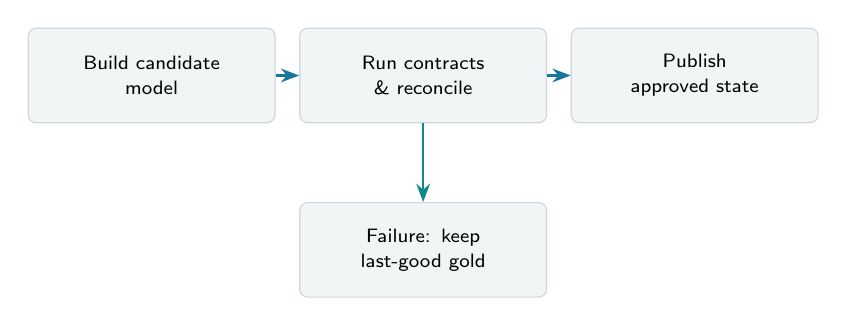
\begin{tikzpicture}[>=Stealth,every node/.style={font=\sffamily\fontsize{7.5}{9}\selectfont},n/.style={draw=thinrule,rounded corners=1mm,fill=papergray,align=center,text width=29mm,minimum height=12mm}]
\node[n](a){Build candidate\\model};\node[n,right=3mm of a](b){Run contracts\\\& reconcile};\node[n,right=3mm of b](c){Publish\\approved state};
\draw[->,thick,steelblue](a)--(b);\draw[->,thick,steelblue](b)--(c);
\node[n,below=10mm of b](d){Failure: keep\\last-good gold};
\draw[->,thick,teal](b)--(d);
\end{tikzpicture}\\{\fontsize{8}{9}\selectfont\color{inkgray}Figure 10.3. Publication is gated independently of candidate computation.}\end{center}
For the energy case, suppose a new model accidentally includes the invalid Solar revision of $-5$~MWh. The candidate's negative-value gate should fail. Operators leave the last approved six-row, 66.000~MWh gold result visible, mark it stale as appropriate, and investigate. If the incorrect model was already published, the team follows the rehearsed restore procedure and checks every affected reporting time window.
\begin{lstlisting}[caption={Minimum change-log entry.}]
release: energy-v1.1.0
commit: <reviewed SHA>
model_change: revision filter tightened
approved_by: <named operator>
integration_result: <Snowflake run IDs>
backout: repoint last-good published relation
verify: current_keys=6; fixture_total=66.000 MWh
\end{lstlisting}
A meaningful rollback record also states what \emph{was not} reverted: the persisted raw event history, consumer caches, notification exports or downstream replicated copies may still require remediation. Snowflake Time Travel can provide recovery options for eligible objects within their retention policy, but it is not a universal substitute for backups, migration design or permission-aware rollback.
\begin{insight}\textbf{Failure mode: revert SQL, forget state}\par
A schema or incremental merge may already have changed target data. Treat code revision and data-state restoration as separate tests, with a business-level reconciliation after both.\end{insight}
\textbf{Check.} Which rollback method preserves a legitimate late correction that arrived after the last code release?
\newpage
% PAGE 188
\topic{10.9.3}{Handover documentation and incident response}
The person paged at midnight needs a map of the pipeline, not a list of folder names. A usable handover names the operating owner, source contact, most important data contract, critical model identifiers, schedule, alert thresholds, typical failure modes, escalation path and manual recovery steps. It distinguishes what can be rerun without data corruption from actions that require explicit approval.
\begin{whitebox}\textbf{Incident scenario: stale daily energy total}\par
\textbf{Signal:} approved gold publication exceeds its freshness objective. \textbf{Triage:} inspect source arrival, validation rejects, dbt run results and task/orchestrator history. \textbf{Containment:} keep last known-good gold result, visibly mark freshness. \textbf{Recovery:} fix input/configuration, stage selective replay, rerun tests, reconcile affected UTC intervals, approve publication. \textbf{Postmortem:} record detection delay, data impact, corrective action and new regression test.\end{whitebox}
Do not automatically retry every failed action. A transient network error may warrant a bounded retry with backoff. A repeated duplicate-key violation is a contract problem, and another ten retries merely spend credits. A permission failure may reflect an intentional policy change; do not escalate to \texttt{ACCOUNTADMIN} as an emergency workaround.

\textbf{The runbook is itself a product artifact.} Store it with the reviewed release, link it from monitoring and test its major steps in an isolated environment. Record the last time an operator verified those steps. Keep the incident procedure small enough to follow under pressure, with detailed technical commands in a controlled supplement.
\begin{lstlisting}[caption={Operator's quick triage, in order.}]
1. Check data contract and expected gold SLA.
2. Identify last successful model and source batch.
3. Inspect failed tests and affected business keys.
4. Determine whether retry/replay is idempotent.
5. Keep or restore last known-good publication.
6. Request approval, rebuild, reconcile, document.
\end{lstlisting}
\repo{P120: Snowflake DevOps data projects guide}{https://github.com/Snowflake-Labs/sfguide-getting-started-with-devops-data-projects-in-snowflake}
\textbf{Check.} What evidence should an on-call engineer capture before deleting a faulty intermediate relation during recovery? How will consumer teams learn whether the report is stale or incorrect?
\newpage
% PAGE 189
\section*{10.L\quad Guided lab, chapter review, and exercises}
\topic{10.L.1}{Prerequisites, inputs, environment, permissions, and cost guardrails}
\textbf{Goal.} Deliver a governed \texttt{fct\_energy\_hourly} model from the twelve synthetic events used in Chapter~9. The offline route is intentionally free: Python~3.10+ with no cloud credentials. The separate \emph{cloud integration route} requires a permitted Snowflake account, an isolated development database/schema, an auto-suspending warehouse and dbt Core plus a compatible Snowflake adapter. Never use production customer data.

\textbf{Inputs.} \texttt{seeds/energy\_revisions.csv} includes duplicate delivery, valid revision correction, tombstone, invalid negative measure and invalid revision. The contract expects six visible current facts and a total of \textbf{66.000~MWh}. These are synthetic assertions, not measurements of Finnish electricity production.
\topic{10.L.2}{Step-by-step procedure with selected code and actual or clearly illustrative results}
\begin{enumerate}
\item Open \texttt{lab/README.md}. Run \texttt{python offline\_oracle.py} and the automated tests. Save \texttt{output/offline\_summary.json}.
\item Inspect the dbt seed and dependency chain: \texttt{stg\_energy\_events} $\to$\\ \texttt{int\_energy\_current} $\to$ \texttt{fct\_energy\_hourly}. Identify the rule that prevents deleted keys from appearing in gold.
\item Examine \texttt{models/schema.yml} and the singular SQL assertions; distinguish domain, uniqueness and fixture-total checks.
\item Review \texttt{offline-checks.yml} and \texttt{manual-cloud-deploy.yml}. Explain why no pull-request workflow holds production secrets.
\item \emph{Optional, approved account only:} configure a personal profile, seed in a disposable schema, run selected \texttt{dbt build}, inspect the result and capture real query/run identifiers. This step has \textbf{not} been performed for this manuscript.
\end{enumerate}
\begin{lstlisting}[caption={Safe zero-cloud commands.}]
cd lab
python offline_oracle.py
python -m unittest -v test_pipeline.py
# Cloud steps are separately approval-gated.
\end{lstlisting}
\begin{whitebox}\textbf{Expected fixture outcome, not a live Snowflake measurement}\par
Delivered events: \textbf{12}. Rejected invalid deliveries: \textbf{2}. Duplicate deliveries: \textbf{1}. Approved current facts: \textbf{6}. Grand total: \textbf{66.000 MWh}. A release fails if any required invariant differs. Read the generated machine-readable summary rather than copying these figures into an operational report.\end{whitebox}
\textbf{Cost guardrail.} Offline execution generates no Snowflake spend. For an actual integration test, agree on expected warehouse usage and teardown before enabling credentials; suspend compute and remove only the disposable objects you own.
\newpage
% PAGE 190
\topic{10.L.3}{Expected result, assertions, common failure diagnosis, rollback, and cleanup}
The acceptance suite tests revision ordering, duplicate delivery, logical deletion, negative-energy quarantine, missing keys, conflicting revisions, idempotent replay, current-row uniqueness, total reconciliation, unit semantics, output manifest and release-gate behaviour. An offline pass demonstrates the \emph{Python contract implementation}; it does not establish that dbt SQL compiled or executed on Snowflake.
\begin{center}\renewcommand{\arraystretch}{1.10}\begin{tabularx}{\linewidth}{@{}p{33mm}X@{}}\toprule
\textbf{Failure symptom}&\textbf{Diagnosis / action}\\\midrule
Duplicate current key&Check event-ID dedupe and revision partition\\
Incorrect total&Compare approved event set and tombstones\\
Missing dbt relation&Review profile, schema generation, grants\\
Stale source&Check ingest time separately from gold publication\\
CI green, cloud red&Review adapter, permissions, role and SQL compile\\\bottomrule\end{tabularx}\end{center}
\textbf{Rollback and cleanup.} The offline lab only writes files in \texttt{lab/output}; deleting that directory restores a clean local state. In a cloud run, use the project-specific approved cleanup plan. Never make a blanket \texttt{DROP DATABASE} command the default teaching step. Save generated manifests, run result artifacts and an operator-approved release note first.
\topic{10.L.4}{Foundation exercise, practitioner exercise, production-design question, and scoring rubric}
\textbf{Foundation (20 pts):} describe the dbt dependency graph and explain why a bronze row may be rejected. \textbf{Practitioner (35 pts):} modify a valid technology revision, recompute the expected six-row current state and update the contract test without weakening quality rules. \textbf{Architecture (30 pts):} propose an environment design, CI gates, freshness thresholds and rollback for an hourly operational dashboard. \textbf{Evidence (15 pts):} provide clean test logs, a reviewed commit hash, a concise ADR and explicit limitations. \emph{Pass guideline:} at least 80/100 with no critical correctness or safety failure.
\begin{insight}\textbf{Chapter synthesis}\par
ETL and ELT determine a transformation boundary; bronze, silver and gold determine data responsibilities; dbt makes models and their dependencies inspectable; orchestration schedules work; CI and contracts guard changes; and release operations protect the users of published data. A reliable data product needs all of these responsibilities assigned, even when no single vendor tool implements them all.\end{insight}
\textbf{Further reading.} \href{https://docs.getdbt.com/docs/build/incremental-models}{dbt incremental models}; \href{https://docs.getdbt.com/docs/build/data-tests}{dbt data tests}; \href{https://docs.getdbt.com/docs/deploy/source-freshness}{dbt source freshness}; \href{https://docs.snowflake.com/en/user-guide/tasks-intro}{Snowflake Tasks}; the research repository URLs noted by section (not independently executed). Verify versions before publication.
\textbf{Next.} Chapter~11 takes tested gold models into semantic definitions and Power BI consumption without losing provenance or grain.
\end{document}
